%%%%%%%%%%%%%%%%%%%%% chapter1.tex %%%%%%%%%%%%%%%%%%%%%%%%%%%%%%%%%
%
%  
%
% Use this file as a template for your own input.
%
%%%%%%%%%%%%%%%%%%%%%%%% Springer-Verlag %%%%%%%%%%%%%%%%%%%%%%%%%%
%\motto{Use the template \emph{chapter.tex} to style the various elements of your chapter content.}






\section{Summary of Module}
\label{sec:1}

 We are interested in approaches to the fundamental hardness questions in computational complexity.

Computational complexity: the study of which problems can be efficiently computed and which cannot.

Efficiency: we understand efficiency as Polynomial Time computability. A Boolean function $f:\{0,1\}^n\to\{0,1\}$ is said to be efficiently computable if there is a polynomial-time Turing Machine M that, on input $x$ in $\bits^n$ outputs $f(x)$ and runs in time $n^c$ for some constant $c$. Note that $n^c$ is a polynomial in the input length $n$ (the exponent $c$ does not depend on the input length $n$). 

The arguably main question of the theory of computation, the one that subsumes in some sense many problems in other parts of computing, once is the \P~vs~\NP~question: Can we separate \P~from \NP, namely, is there a language in \NP~ that is not in \P? In other words, can we prove that SAT (Boolean satisfiability problem) cannot be solved in polynomial time? And yet again, roughly, can problems whose solutions once given can be verified efficiently, can be solved efficiently? 

We are interested in \emph{concrete} approaches, namely, considering a simple, usually combinatorial-looking, model of computation, such as a Boolean circuit, and establishing lower bounds against the size of circuits required to prove certain specific functions that are given to us concretely (usually, these functions also possess some straightforward combinatorial 
properties; e.g., they represented specific graph problems). In this sense, the question is concrete because the result is unconditional (namely, it does not depend on unproved 
assumptions, such as $\P\neq\NP$), and the model itself is concrete: it is a (primarily combinatorial) object of which its size we lower 
bound in precise terms (e.g., circuit $C$ computing function $f(x)$ must have size $2^{|x|}$, where $|x|$ is the bit-size of the input $x$).
\medskip 

Three main concrete approaches to the fundamental hardness questions are the following:

\begin{enumerate}
\item  Circuit Complexity 
\item Proof Complexity 
\item Algebraic Complexity
\end{enumerate}

We shall see a bit from each, mainly circuit complexity and some basic proof complexity while commenting briefly on algebraic complexity. 



Other approaches to the fundamental hardness questions are usually more intrinsic to complexity theory. In that respect, the whole of computational complexity theory could be viewed as ``approaching" the fundamental hardness questions through complexity class, reductions, concrete lower bounds and the relation between these notions and results. One intriguing approach that makes this attempt in particular is the ``Meta Complexity" approach. We are not going to touch on this in this course. 



\chapter{Introduction to Circuit Complexity}
\label{intro} % Always give a unique label
% use \chaptermark{}
% to alter or adjust the chapter heading in the running head
 

\section{Basic Circuit Complexity}
\label{sec:2}
% Always give a unique label
% and use \ref{<label>} for cross-references
% and \cite{<label>} for bibliographic references
% use \sectionmark{}
% to alter or adjust the section heading in the running head

\begin{definition}[Boolean Circuit]
Let $n \in \mathbb{N}$ and $x_1, \ldots, x_n$ be $n$ variables. A Boolean Circuit $C$ with $n$ inputs is a directed acyclic graph. It contains $n$ nodes with no incoming edges, called the \emph{input nodes} and a single node with no outgoing edges, called the \emph{output node}.
All other nodes are \emph{internal nodes} or \emph{gates}, and
are labelled by the logical gates $\lor, \land,\neg$ (i.e., logical OR, AND, NOT, resp.). The $\lor,\land$ nodes have fan-in (i.e., number of incoming nodes) 2, and $\neg$ has fan-in 1. The \emph{size of $C$}, denoted $|C|$, is the number of nodes in the underlying graph.
$C$ is called a \emph{formula} if each node has at most one outgoing edge (i.e., the underlying graph is a tree),
\end{definition}




\begin{figure}
\sidecaption
  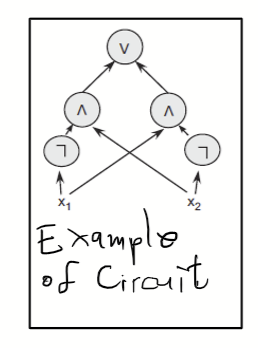
\includegraphics[width=0.2\linewidth]{images/Example-circuit.png}
    \caption{Example of a simple Boolean circuit.}
    \label{fig:enter-label}
\end{figure}

%

\subparagraph{Comment}
Fan-in $d>2$ 
can be simulated by a tree of $d-1 $ nodes: 
\begin{figure}[h]
    \centering
  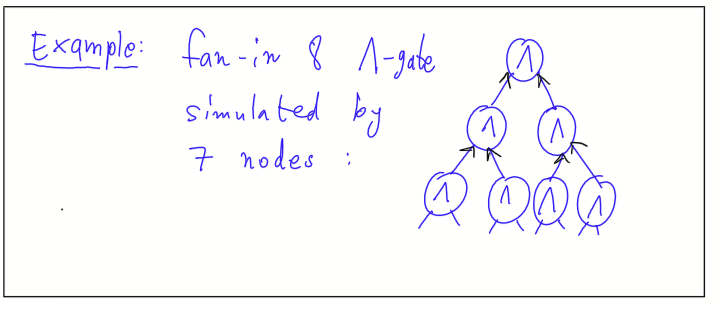
\includegraphics[width=0.5\linewidth]{images/Example-tree-circuit.png}
    \label{fig:enter-label}
\end{figure}
 


\newpage 

\begin{question}{What is the function computed by the circuit below?}
\begin{figure}
    \centering
    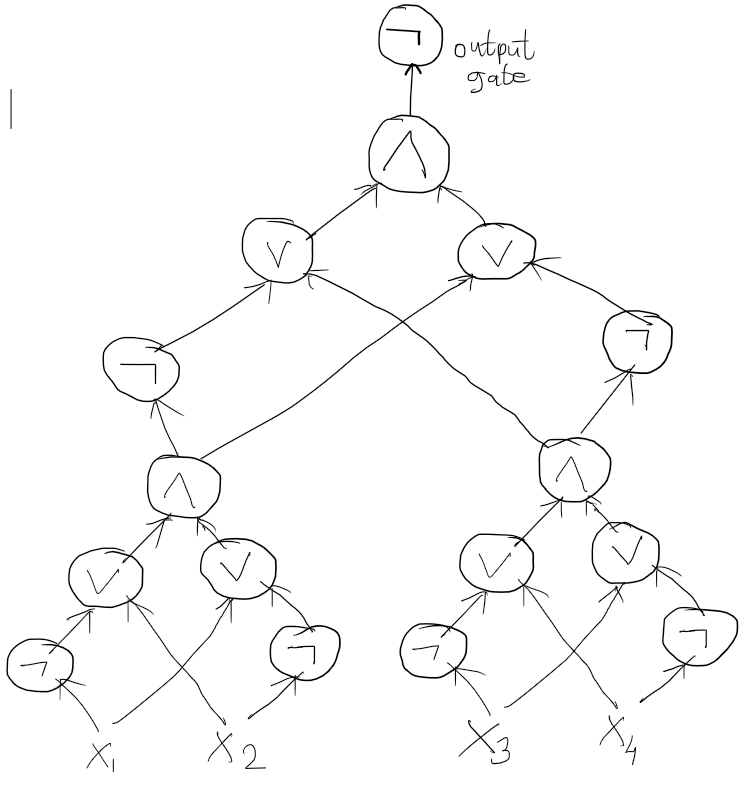
\includegraphics[width=0.75\linewidth]{images/parity-circuit-question.png}
    \caption{Question}
    \label{fig:enter-label}
\end{figure}
\end{question}

\begin{trailer}{Answer}
     PARITY on 4 input bits. It outputs 1 if the number of 1's in the input is odd. I.e., it computes the XOR of $x_1, \ldots, x_4$. In other words, it computes the function $x_1+x_2+x_3+x_4$ mod 2. (Understand why that is. Hint: recall that ${\neg x_1}\lor x_2$ is logically equivalent to $x_1\to x_2$. And notice that this structure repeats throughout the circuit.)
\end{trailer}
%\eject

\section{Circuit families, language recognition, and function computation}

Let $\mathbb{N}$ denote the set of natural numbers starting from $1$.


%\newcommand{\bits}{\ensuremath{\{0,1\}}}
%\newcommand{\demph}[1]{\textbf{\emph{#1}}}

A \emph{language} is a set of (finite) strings. Note that the language can contain infinite many strings, only that each string is finite. A \emph{string} is an ordered sequence of symbols from a fixed constant size alphabet. We shall use mainly strings over the alphabet consisting of two symbols $\bits$.
Hence, a language is simply a set $L\subseteq\bits^*$ (recall, that $\bits^*$ is the set of all finite 0-1 strings, including the empty string). 
 

\begin{svgraybox}
\begin{definition}
Let $T:\mathbb{N}\rightarrow \mathbb{N}$ be a function. 
A \emph{$T(n)$-\textbf{sized circuit family}} is a sequence $\left\{C_n\right\}_{n \in \mathbb{N}}$ of Boolean circuits, where $C_n$ has $n$ input-gates (i.e., $n$ inputs-bits) and a single output-bit such that  $\left|C_n\right| \leq T(n), \forall n \in \mathbb{N}$.\footnote{We can also define a circuit-family where some input lengths $n\in\mathbb{N}$ are \emph{skipped} in the sequence, e.g., if the length of every input should be even. We shall not use this subtlety here.}
\end{definition}
\end{svgraybox}

A language $L\subseteq\{0,1\}^*$ is said to be \emph{in} $\operatorname{\SIZE} (T(n))$, namely, $$L\in\operatorname{\SIZE} (T(n)),$$ if there is a $T(n)$-size circuit family $\left\{C_n\right\}_{n \in \mathbb{N}}$ s.t. (such that) 
$$\forall n \in \mathbb{N~} \forall x \in\{0,1\}^n: x \in L \Leftrightarrow C_n(x)=1.$$
In this case, we say that 
the family $\left\{C_n\right\}_{n \in \mathbb{N}}$ \demph{decides} the language $L$.


Similarly, for a \emph{function} $f:\{0,1\}^* \rightarrow\{0,1\}, f \in \operatorname{\SIZE}(T(n))$ if there exists $ T(n)$-size circuit family $\left\{C_n\right\}_{n \in \mathbb{N}}$ such that  $\forall n \in \mathbb{N} \quad \forall x \in\{0,1\}^n, f(x)=1 \Leftrightarrow C_n(x)=1$.
In this case, we say that 
the family $\left\{C_n\right\}_{n \in \mathbb{N}}$ \demph{computes} the function $f$.



\begin{svgraybox}
\textbf{Slice of function}. 
 Let $f:\{0,1\}^*\to\{0,1\}$ be a Boolean function.
We can consider the \emph{slice} \emph{of size} $n$ of $f$ to be the function $f_n:\{0,1\}^n\to\{0,1\}$, which is $f$ restricted to inputs of length precisely $n$. 
\end{svgraybox}

Similarly, we can consider $\left\{f_{n}\right\}_{n\in\mathbb{N}}$ to be the \textit{family} of Boolean functions $f_n:\{0,1\}^n\to \{0,1\}$, 
for all $n$ at least 1 (so, this is a family of all slices of $f$). In other words, the family $\left\{f_{n}\right\}_{n\in\mathbb{N}}$ is the sane as $f:\bits^*\to\bits$. 

\textcolor{green}{STOPPED polish Here
}






\section{Quick recap:\ growth functions, $O$-notation and run-times}

Be sure to recall the following basic definitions of (though we are not going to use them concretely in this course).

- Time bounds for Turing Machines (TMs)

- The class P (aka PTIME)

- The class NP, verifiers, short certificates

- SAT is NP complete: Cook-Levin theorem



\paragraph{Time Complexity}
We mainly consider the worst-case time for a problem to be solved by a given TM.

\begin{definition}
    Let $M$ be a $T M$ that halts on every input. Let $f: \mathbb{N} \rightarrow \mathbb{N}$ be a function, s.t., $f(n)$ is the max number  of steps it takes $M$ to halt on inputs of length $n$. We say $f$ is the running time of $M$. And that $M$ runs in time $f(n)$.
\end{definition}

\begin{trailer}{$O$-Notation}
    We usually use $n$ for the length of inputs


Recall:
\begin{enumerate}
    \item 
 $f(n)=O(g(n))$ if $\exists$ constant $c$ and $n_0 \in \mathbb{N}$ st. $\forall n \geqslant n_0 \quad f(n) \leqslant c g(n) $ (for two functions  $f, g: \mathbb{N} \rightarrow \mathbb{R}^{+}$).

\item $f(n)=o(g(n))$ if $\lim _{n \rightarrow \infty} \frac{f(n)}{g(n)}=0$
\end{enumerate}
\end{trailer}

\begin{trailer}{Basic Growth Rates}
\begin{enumerate}
    \item When $f=O\left(\log n\right)$ the base $b$ of $\log _b n$ is irrelevant.
    
    \item $2^{O(n)}$ means $\leqslant 2^{c n}$ for some $c$, const.

    \item \emph{Polynomial growth rate} means $n^{O(1)}=2^{O\left(\log n\right)}=n^c$, for some constant $c$, namely $c$ is independent of $n$ (while $n$ grows, $c$ stays fixed).
    \item \emph{Exponential growth rate} (similarly, \emph{exponential bound})  means for us $2^{n^\delta}$, for a real constant $\delta>0$. (Some texts insist that ``exponential growth'' should only refer to $2^{cn}$, for a constant $c>0$. Note the difference between this and our definition!)
\end{enumerate}
\end{trailer}






\begin{definition}[\Ppoly; polynomial-size circuits] The class \Ppoly~is the class of languages that are decidable by polynomial-size circuit families.
That is, $\Ppoly=\bigcup_{c \in \mathbb{N}} \operatorname{\SIZE}\left(n^c\right)$.
\end{definition}


\begin{theorem}
$\P \subseteq \Ppoly$.
\end{theorem}

\begin{proof}
Assignment/tutorial.
[See for a sketch in Arora-Barak'10, Sec. 6.1.1. page 110; \cite{AB09}]. 
\end{proof}

\section{Our main focus: lower bounds}

\begin{svgraybox}
\textbf{Lower bounds, hard functions}.
We say that we have a \textit{super-polynomial lower bound against \Ppoly}, namely a super-polynomial lower bound against (polynomial-size) Boolean circuits, if the following occurs: there exists a Boolean function $f:\{0,1\}^*\to \{0,1\}$ such that no polynomial-size circuit family $\left\{C_n\right\}_n$ computes $f$. In other words, $f$ is not in $\Ppoly$. If we show that $f\not\in\operatorname{\SIZE}(T(n))$, we say that we have \textit{proven a $T(n)$-lower bound for $f$} (against Boolean circuits). We say that this $f$ is \emph{hard} for $\operatorname{\SIZE}(T(n))$.
\end{svgraybox}



\paragraph{Motivation for Circuit Complexity}

1)  Non-uniformity: maybe for every $l \in \mathbb{N}$ there's a small circuit for SAT that can solve it in quadratic time?
(Karp-Lipton: PH doesn't collapse $\Rightarrow N P \subseteq P /$ poly).

2) Mathematically \textit{cleaner} than Turing Machines; so might have better hope for lower bounds.


\subsection{Most functions are hard: Shannon lower bound}

\begin{figure}
    \centering
    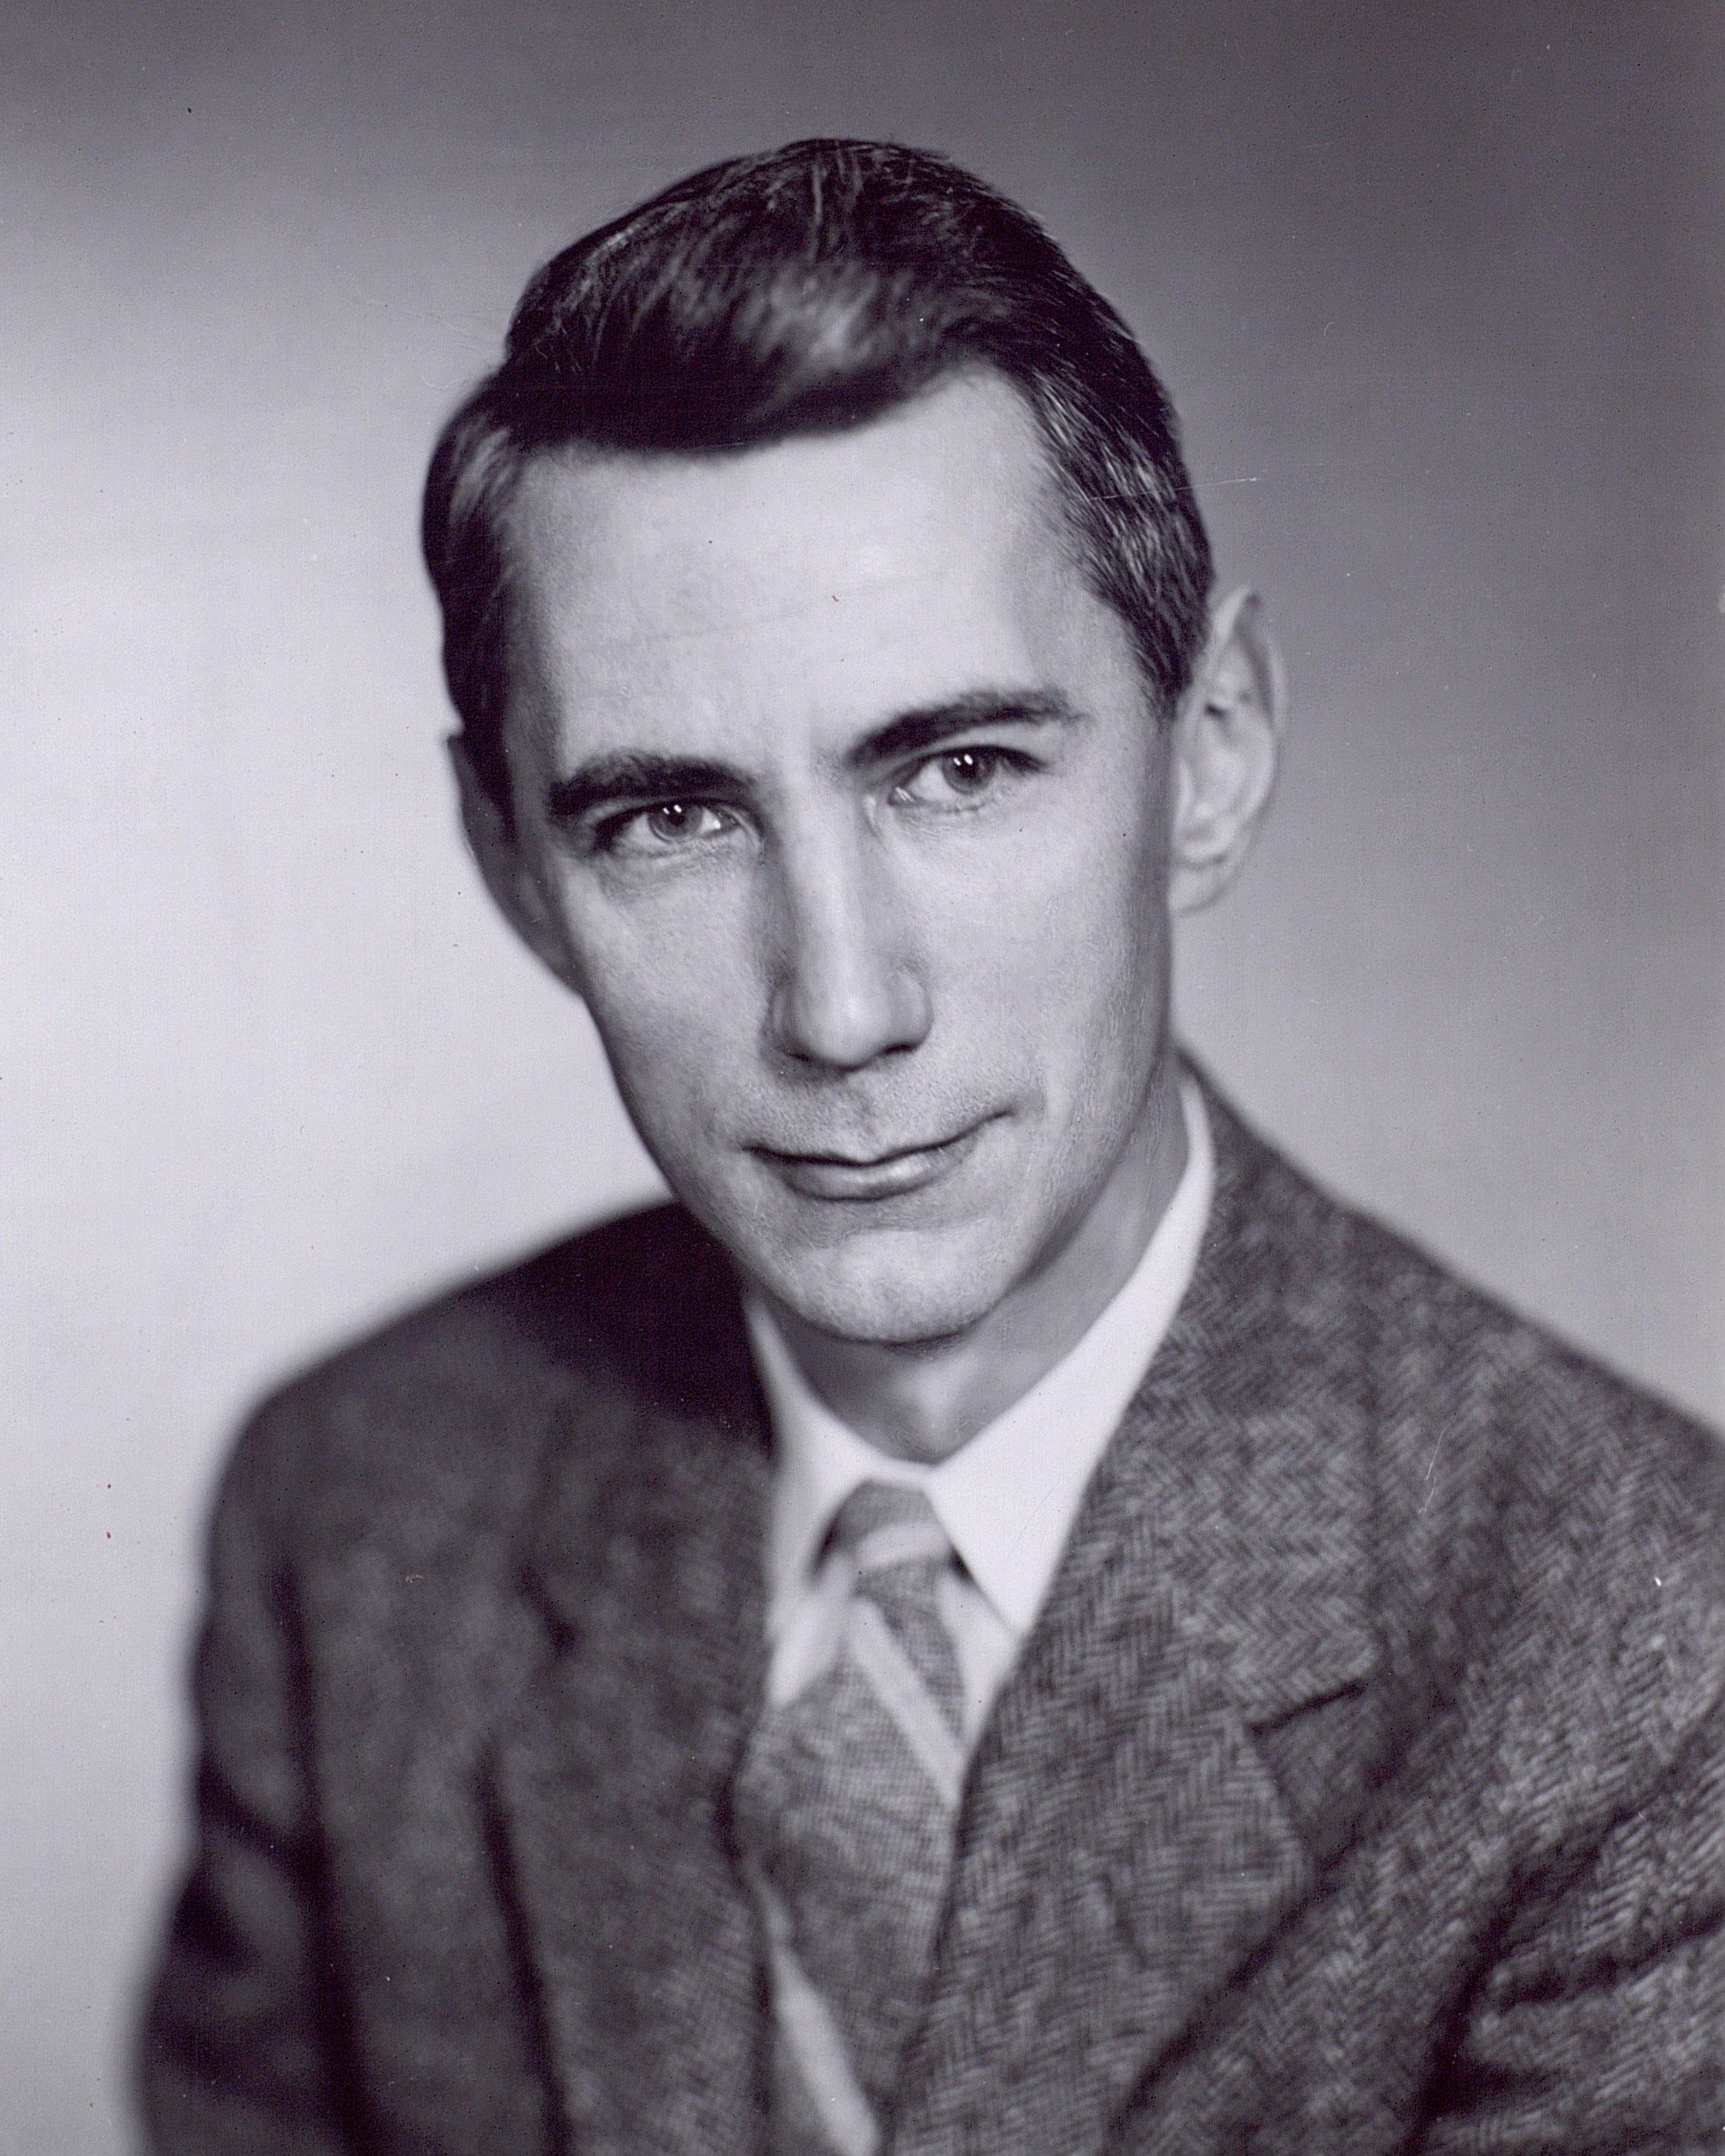
\includegraphics[width=0.25\linewidth]{images/Shannon.jpg}
    \caption{C.E.~Shannon. Source: By Unknown author - Tekniska Museet, CC BY 2.0, \url{https://commons.wikimedia.org/w/index.php?curid=144716444}}
    \label{Claude Shannon}
\end{figure}






Open: $\quad \mathrm{NEXP}\stackrel{?}{\subseteq}P/poly$ (note that by the time hierarchy theorem $\mathrm{EXP}\subsetneq P$; but in ``$\mathrm{NEXP}\stackrel{?}{\subseteq}P/poly$'' we consider NEXP which is \emph{uniform}, and P/poly which is \textit{non}-uniform).


\begin{theorem}
    [Shannon lower bound]
    For every $n>1$ exists a function $f:\{0,1\}^n \rightarrow\{0,1\}$ that cannot be computed by a circuit of size  $\le 2^n / 10 n$.
\end{theorem}

\begin{proof}[by counting method.]
\mbox{}\\

\begin{claim}
We can encode a boolean circuit of size $S$ with $9\cdot S \log S$ bits.
\end{claim}

\begin{proof}[Claim]
Using adjacency List:
\begin{figure}[H]
    \centering
    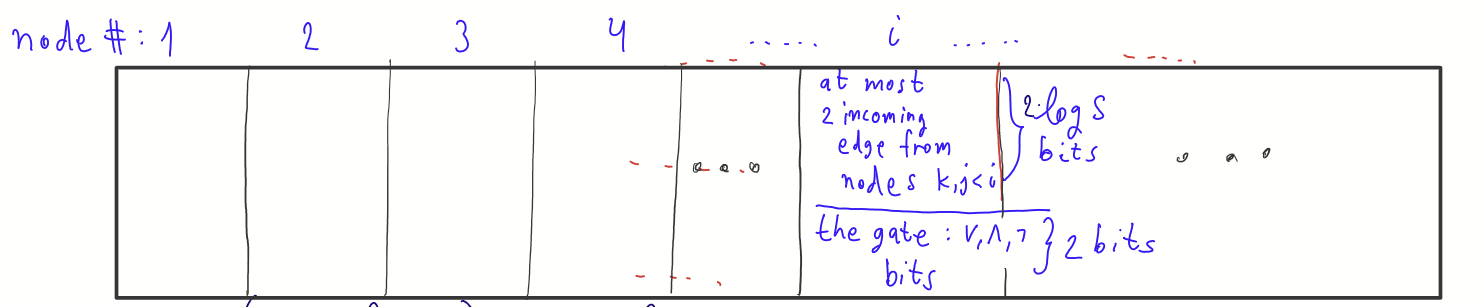
\includegraphics[width=1.1\linewidth]{images/shannon_table.png}
    \caption{Enter Caption}
    \label{fig:enter-label}
\end{figure}




We have:
$$
S \cdot(2+2 \log S) \leq 9 S \log S
.$$
(Actually, we have: 
$ 2S(\log S+1) = 2S(2 \log S) \leq 4 S \log S.
$)
\end{proof}

We now show that the number of circuits of size $\leq 2^n / 10 n$ is smaller than that of possible Boolean functions w/ $n$ inputs.
Thus, by the Pigeonhole Principle, there exists a Boolean function that cannot be computed by a circuit of size $\leq 2^n / 10 n$.

The number of circuits of size $S$ is bounded from above by the number of distinct codes of circuits of size $S$, which is
$$
\begin{aligned}
& \leq 2^{9 \cdot S \log S} \\
& =2^{\left(9 \cdot 2^{n / 10 n} \cdot \log \left(2^n / 10 n\right)\right)}=2^{\left(9 \cdot 2^n / 10 n \cdot(n-\log 10 n)\right)} \\
& \leq 2^{\frac{9 n}{10 n} \cdot 2^n}=2^{\frac{9}{10} \cdot 2^n} . 
\end{aligned}
$$
But this is 
less than $2^{2^n}$ the number of distinct Boolean functions $f:\{0,1\}^n\to\{0,1\}$. 
\end{proof}




Note: the reason we need to lower bound $2^n/10n$ circuits (and not $2^n/c$), is that encoding a circuit is super linear (i.e., $\Omega (\log n)$).



